\section{Patterns 6 - Model-View-ViewModel (MVVM)}

\subsection{Fokuspunkter}

\begin{itemize}
	\item Redegør for, hvad et software pattern er.
	\item Redegør for Model-View-ViewModel mønstret og dets variationer.
\end{itemize}

\subsection{Hvad er et Software pattern?}

\derp

Dette design pattern, er et GUI architecture pattern, som er en specaialisering af Model-View-Presenter møsntret.

\subsection{Redegør for Model-View-ViewModel mønstret og dets variationer}

\begin{figure}[h]
	\centering
	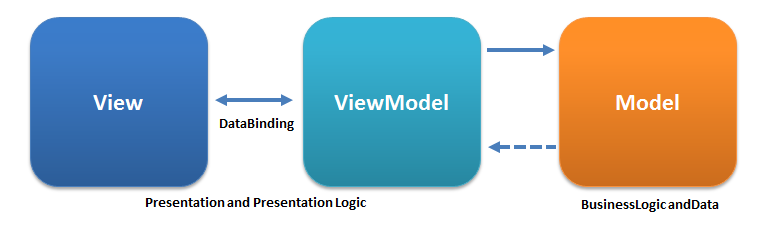
\includegraphics[width=0.7\linewidth]{figs/MVVM/MVVMPattern.png}
	\caption[Sammenhæng mellem Model-View-ViewModel]{}
	\label{fig:MVVMPattern}
\end{figure}

\subsubsection{View}

\begin{enumerate}
	\item User Interface.
	\item Definerer struktur, layout og appearance.
	\item Ideelt er det udelukkende defineret i XAML, med begrænset "code behind" som \textbf{\textit{ikke}} indeholder business logic.
	\item Kan være en subcomponent af et andet view.
	\item Kan have sin egen ViewModel eller arve dens parents.
	\item Viewet får data fra ViewModel gennem \textbf{\textit{databinding}} eller metodekald på ViewModel
	\item View ændres \textbf{\textit{run-time}} når UI controls\todo{what is dis?}, agerer efter ændringer i ViewModels properties.
	\item Hvad sker der der laves User Input på View?
	\begin{itemize}
		\item Hvis control er en \textbf{\textit{Command Source}} kan control's Command property være data bound til en ICommand property på view model.
		\item View er connected til ViewMOdel gennem databinding og sender commands to ViewModel
	\end{itemize}
\end{enumerate}

\subsubsection{ViewModel}
\begin{enumerate}
	\item \textbf{En model af Viewet}.
	\begin{itemize}
		\item En abstraktion af viewet der leverer \textbf{data binding} mellem View og Model
		\item En specialiseret udgave af MVP's presenter (agerer også \textit{converter} der omdanner Model data til View data), og samtidig overfører commands fra View til Model.
	\end{itemize}
	\item ViewModel har \textbf{\textit{public}} properties og commands.
	\item  Interagerer med Model gennem Databinding, properties og metodekald.
	\item Modtager events fra Model
\end{enumerate}

\subsubsection{Model}
\begin{enumerate}
	\item Refererer som i MVC til enten:
	\begin{itemize}
		\item Object-model, der repræsenterer state content.
		\item Data Access layer der repræsenterer indhold.
	\end{itemize}
	\item \textbf{Kender ikke til ViewModel}\todo{hvordan sender den events?}
	\item Sender evnets til ViewModel
\end{enumerate}

\begin{figure}[H]
\centering
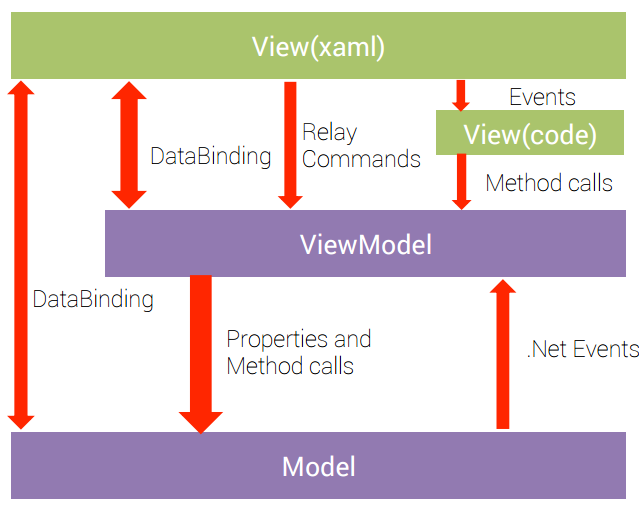
\includegraphics[width=0.7\linewidth]{figs/MVVM/mvvmPatternComplex}
\caption{Intern adfærd i MVVM pattern}
\label{fig:mvvmPatternComplex}
\end{figure}


\subsubsection{Hvorfor er det smart?}

\begin{itemize}
	\item \textbf{Test uden UI} - UI indeholder ikke business logic.
	\item 
\end{itemize}




